\section*{Section~\ref{S:setoperations}}

\subsection*{Progress Check~\ref{prog:setnotation}}
\begin{center}
\begin{tabular}{r p{0.8in} l p{0.5in} r p{0.8in} l }
  $A$   & $\not \subset, \not \subseteq \ne$  & $B$   &   & $\emptyset$   & $\subset, \subseteq, \ne$  & $A$ \\ \cline{2-2} \cline{6-6}
   5    & $\in$  & $B$   &   &  $\left\{ 5 \right\}$     & $\subset, \subseteq, \ne$ &  $B$ \\ \cline{2-2} \cline{6-6}
  $A$   & $\ne$  & $C$   &   &  $\left\{ {1,2} \right\}$  & $\ne$  &  $C$ \\ \cline{2-2} \cline{6-6}
  $\left\{ {1,2} \right\}$ & $\subset, \subseteq, \ne$ &  $A$ &  &  $\left\{ {4,2,1} \right\}$ & 
$\subseteq, =$ & $A$ \\ \cline{2-2} \cline{6-6}
  6     & $\notin$ &  $A$ &  &  $B$  & $\ne$  & $\emptyset$ \\ \cline{2-2} \cline{6-6}
\end{tabular}
\end{center}



\subsection*{Progress Check~\ref{prog:venndiagrams}}
\begin{enumerate}
  \item \begin{multicols}{2}
\begin{center}
\scalebox{0.6}{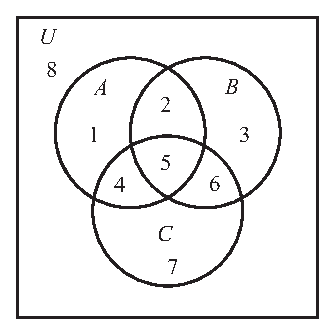
\includegraphics{figps-venn3.eps}}
\end{center}
Using the standard Venn diagram for three sets shown above:
\begin{enumerate}
  \item For the set $(A \cap B) \cap C$,  region 5 is shaded.
  \item For the set $(A \cap B) \cup C$, the regions 2, 4, 5, 6, 7 are shaded.
  \item For the set $(A^c \cup B)$, the regions 2, 3, 5, 6, 7, 8 are shaded.
  \item For the set $(A^c \cap (B \cup C))$, the regions 3, 6, 7 are shaded.
\end{enumerate}
\end{multicols}

\begin{multicols}{2}
\item \begin{center}
\scalebox{0.8}{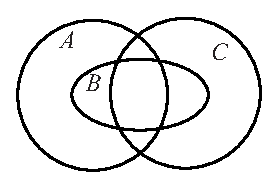
\includegraphics{figps-prog54-2.eps}}
\end{center}

\item \begin{center}
\scalebox{0.8}{
\includegraphics{figps-prog54-3.eps}}
\end{center}
\end{multicols}

\end{enumerate}
%\hbreak



\endinput
